%! Author = Juniell
%! Date = 31.05.2021

% Preamble
\documentclass[a4paper, 14pt]{extarticle}

% Packages
\usepackage[T2A]{fontenc}
\usepackage{natbib}
\usepackage{graphicx}
\usepackage[english, russian]{babel}
\usepackage{fontspec}
\usepackage{amsmath}
\usepackage{amsfonts}
\usepackage{amssymb}
\usepackage{amsthm}
\usepackage{mathtools}
\usepackage{mathrsfs}
\usepackage{fullpage}
\usepackage{ulem}
\usepackage{setspace}
\usepackage{listings}
\usepackage{indentfirst}
\usepackage[left=2cm,right=1.5cm,top=2cm,bottom=2cm]{geometry}
\usepackage{xcolor}
\usepackage{float}
\usepackage{csquotes}
\usepackage{hyperref}
\usepackage{graphics}

\definecolor{urlcolor}{HTML}{0000FF} % цвет ссылок
\definecolor{linkcolor}{HTML}{000000} % цвет гиперссылок
\hypersetup{pdfstartview=FitH, linkcolor=linkcolor, urlcolor=urlcolor, colorlinks=true}

\setmainfont{Times New Roman}
\setlength{\parindent}{5ex}
\setlength{\parskip}{1em}
\renewcommand{\baselinestretch}{1}

\graphicspath{{resources/Images}}

\definecolor{buzzlightyear}{HTML}{8757A5}
\definecolor{grass}{HTML}{738D06}
\definecolor{literal}{HTML}{F18A2B}
\definecolor{commentcolor}{HTML}{8E908B}

\lstdefinestyle{habrstyle}{
    backgroundcolor=\color{white},
    commentstyle=\color{commentcolor},
    keywordstyle=\bfseries\color{buzzlightyear},
    numberstyle=\tiny\color{commentcolor},
    stringstyle=\color{grass},
    basicstyle=\ttfamily\footnotesize,
    breakatwhitespace=false,
    breaklines=true,
    captionpos=b,
    keepspaces=true,
    numbers=left,
    numbersep=5pt,
    showspaces=false,
    showstringspaces=false,
    showtabs=false,
    tabsize=4,
    language=Python
}

\lstset{style=habrstyle}

% Document
\begin{document}
% Титульный лист
    \begin{center}
        \begin{center}
            \hfill \break
            \normalsize{Санкт-Петербургский государственный политехнический}\\
            \normalsize{университет Петра Великого}\\
            \hfill \break
            \normalsize{\textbf{Высшая школа интеллектуальных систем и}}\\
            \normalsize{\textbf{суперкомпьютерных технологий}}\\
            \hfill \break
            \hfill \break
            \hfill \break
            \hfill \break
            \hfill \break
            \normalsize{Отчёт по лабораторной работе №12}\\
            \normalsize{Дисциплина: Телекоммуникационные технологии}\\
            \normalsize{Тема: GNU Radio}\\
        \end{center}
        \hfill \break
        \hfill \break
        \hfill \break
        \hfill \break
        \hfill \break
        \hfill \break
        \hfill \break
        \hfill \break
        \hfill \break
        \hfill \break
        \begin{tabbing}
            Выполнил студент гр. 3530901/80201 \`В.А. Пучкина\\
            \\
            Преподаватель: \`Н.В. Богач\\
        \end{tabbing}
        \hfill \break
        \hfill \break
        \hfill \break
        \hfill \break
        \begin{center}
            Санкт-Петербург\\
            2021
        \end{center}
        \thispagestyle{empty}
    \end{center}

% Оглавление
    \newpage
    \tableofcontents

% Список иллюстраций
    \newpage
    \listoffigures

% ---------------------------------------------- Передача сигнала ----------------------------------------------
    \newpage
    \section{Передача сигнала}
    \label{sec:task1}

    Первый этап - передача сигнала QPSK. Генерируется поток битов и модулируется на сложное созвездие.
    Для этого используется блок Constellation Modulator, который использует Constellation Rect. Object и другие
    настройки для управления передаваемым сигналом.

    Объект созвездия позволяет определить, как кодируются символы.
    Блок модулятора может использовать эту схему модуляции с дифференциальным кодированием или без него.
    Модулятор созвездия ожидает упакованные байты, поэтому используется генератор случайного источника, предоставляющий
    байты со значениями 0-255.

    Чтобы обеспечить желаемую скорость передачи данных, количество выборок на символ должно быть минимальным.
    При моделировании это значение важно только для того, чтобы обеспечить соответствие этой скорости по всей
    потоковой диаграмме.
    Мы будем использовать количество выборок на символ равное 4.
    Это больше, чем нужно, но полезно для визуализации сигнала в различных областях.

    Наконец, мы устанавливаем значение избыточной пропускной способности.
    Поточный график (\texttt{flowgraph}) mpsk\_rrc\_rolloff.grc (Рис.\ref{fig:task1_flowgraph}) генерирует следующий
    рисунок (Рис.\ref{fig:task1_excess_bandwidth}), показывающий различные значения избыточной пропускной способности.

    \begin{figure}[H]
        \centering
        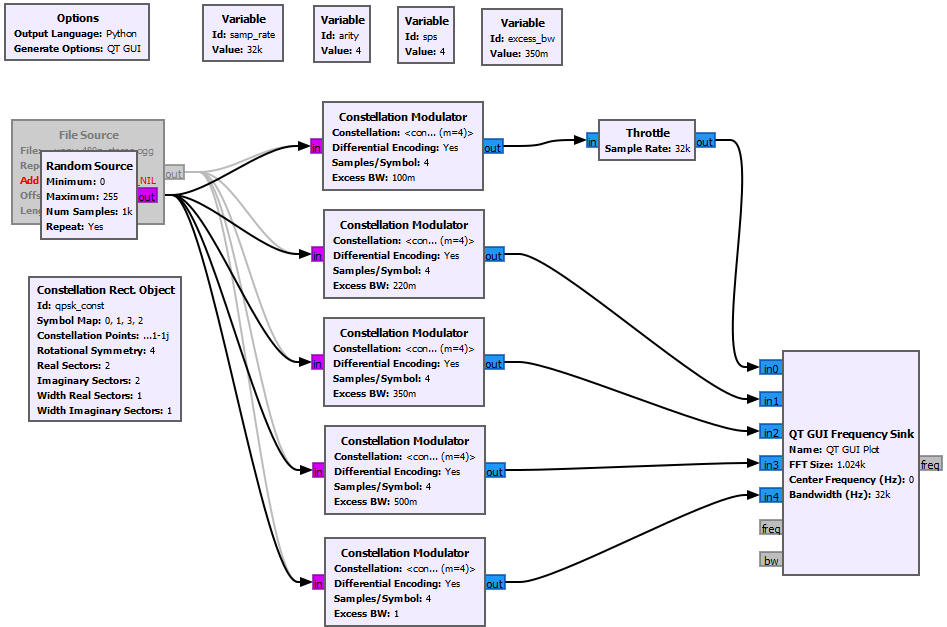
\includegraphics[width=0.75\linewidth]{resources/Images/task1_mpsk_rrc_rolloff}
        \caption{Flowgraph mpsk\_rrc\_rolloff.grc.}
        \label{fig:task1_flowgraph}
    \end{figure}

    \begin{figure}[H]
        \centering
        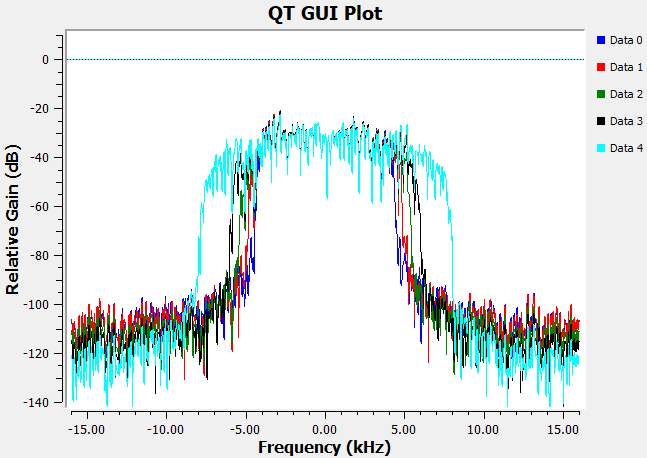
\includegraphics[width=0.8\linewidth]{resources/Images/task1_excess_bandwidth}
        \caption{Избыточная пропускная способность.}
        \label{fig:task1_excess_bandwidth}
    \end{figure}

    Типичные значения находятся в диапазоне от 0,2 (красная кривая) до 0,35 (зеленая кривая).

    Теперь изучим файл \texttt{mpsk\_stage1.grc}, передающий созвездие QPSK.
    Его \texttt{flowgraph} представлен на Рис.\ref{fig:task1_mpsk_stage1}.

    \begin{figure}[h]
        \centering
        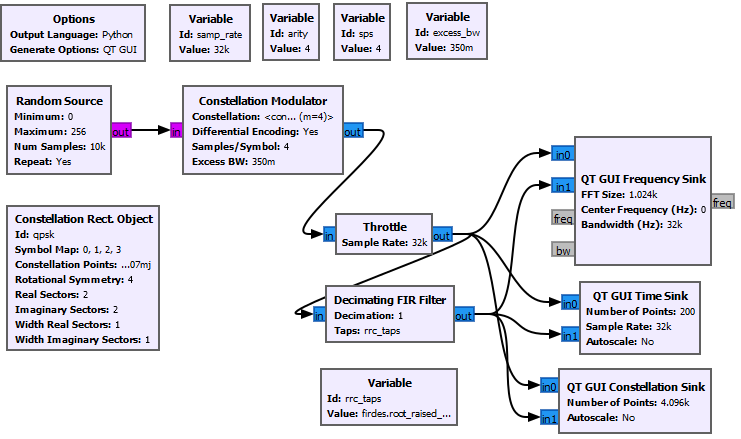
\includegraphics[width=0.8\linewidth]{resources/Images/task1_mpsk_stage1}
        \caption{Flowgraph mpsk\_stage1.grc.}
        \label{fig:task1_mpsk_stage1}
    \end{figure}

    \begin{figure}[h]
        \centering
        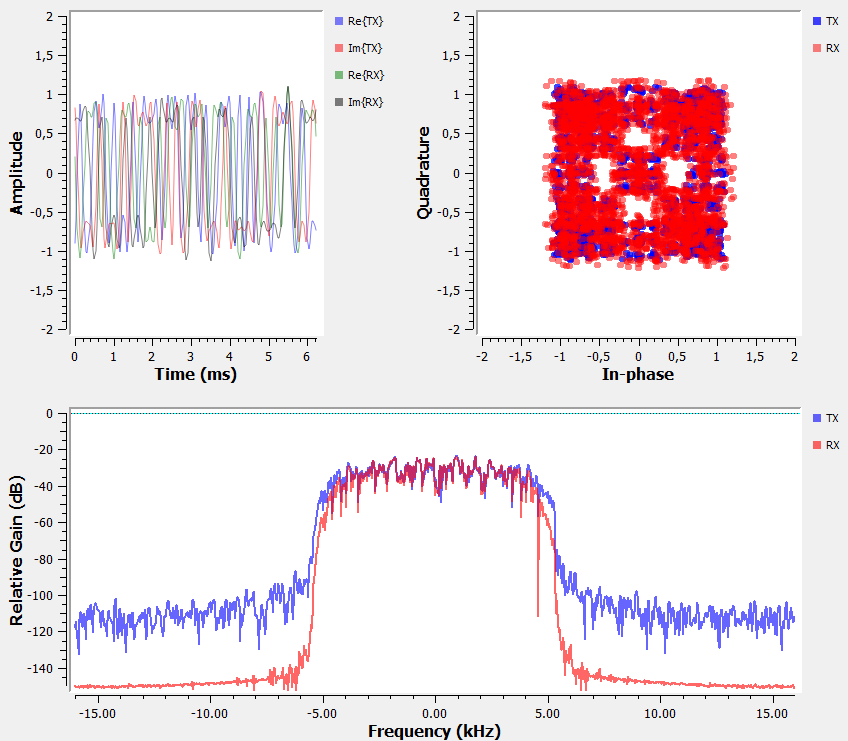
\includegraphics[width=0.8\linewidth]{resources/Images/task1_up_samling}
        \caption{Созвездие QPSK.}
        \label{fig:task1_up_samling}
    \end{figure}

    На графике созвездия можно увидеть эффекты повышающей дискретизации и процесс фильтрации.
    В этом случае фильтр RRC добавляет преднамеренные самоинтерференции (межсимвольные помехи, ISI).
    Это плохо влияет на принимаемый сигнал, потому что символы смешиваются.

    Видно, что частотный график показывает сигнал красивой формы, переходящий в шум.
    Если бы мы не применили формирующий фильтр к сигналу, то передавали бы прямоугольные волны,
    которые производили бы много энергии в соседних каналах.
    Благодаря уменьшению внеполосных излучений теперь сигнал остается в пределах полосы пропускания канала.

    На стороне приема мы избавляемся от ISI с помощью другого фильтра.
    Таким образом, происходит сворачивание двух фильтров RRC вместе.
    В результате получается фильтр с приподнятым косинусом, который является формой фильтра Найквиста.

    Фильтрация является просто сверткой, поэтому выходной сигнал RRC-фильтра на приемной стороне
    представляет собой сигнал в форме приподнятого косинусоидального импульса с минимизированным ISI.
    Другое преимущество состоит в том, что при отсутствии эффектов канала мы используем согласованный фильтр на приемнике.

    \newpage

    % --------------------------------------- Добавление нарушений канала ----------------------------------------------
    \section{Добавление нарушений канала}
    \label{sec:task2}

    Теперь рассмотрим влияние канала и то, как сигнал искажается между моментом передачи и моментом приёма.
    Изучим файл \texttt{mpsk\_stage2.grc}.
    Будем использовать самый простой блок модели канала GNU Radio, позволяющий смоделировать несколько основных проблем,:

    \begin{enumerate}
        \item Шум.
        Тепловой шум в приемнике вызывает аддитивный белый гауссовский шум (AWGN).
        Мы устанавливаем мощность шума, регулируя значение напряжения шума модели канала.
        Можно рассчитать напряжение шума, исходя из желаемого уровня мощности, зная другие параметры моделирования.
        \item Разные \texttt{clock}, которые определяют частоту радиомодулей.
        Грубо говоря, одно радио номинально работает на частоте \texttt{fc}.
        С учётом его недостатков, это означает, что фактически оно работает на частоте \texttt{fc+f\_delta\_1}.
        Другое радио аналогично будет иметь своё смещение - \texttt{f\_delta\_2}.
        Таким образом, полученный сигнал будет смещён на \texttt{f\_delta\_1 + f\_delta\_2}
        \item Идеальная точка выборки.
        Эта проблема связана с предыдущей.
        Два радиомодуля работают с разной скоростью, а потому идеальная точка выборки неизвестна.
    \end{enumerate}

    \begin{figure}[h]
        \centering
        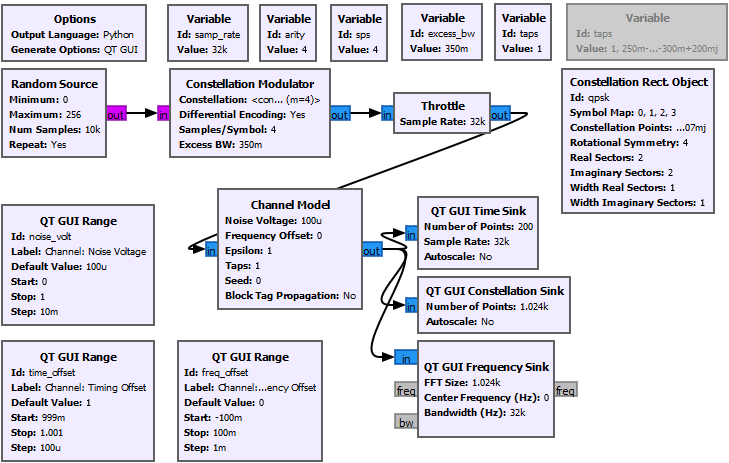
\includegraphics[width=0.8\linewidth]{resources/Images/task2_mpsk_stage2}
        \caption{Flowgraph mpsk\_stage2.grc.}
        \label{fig:task2_mpsk_stage2}
    \end{figure}

    Запустим наш \texttt{flowgraph}.
    Мы можем поэкспериментировать с эффектами аддитивного шума, сдвига частоты и временного сдвига и посмотреть
    на результирующий сигнал.

    \begin{figure}[h]
        \centering
        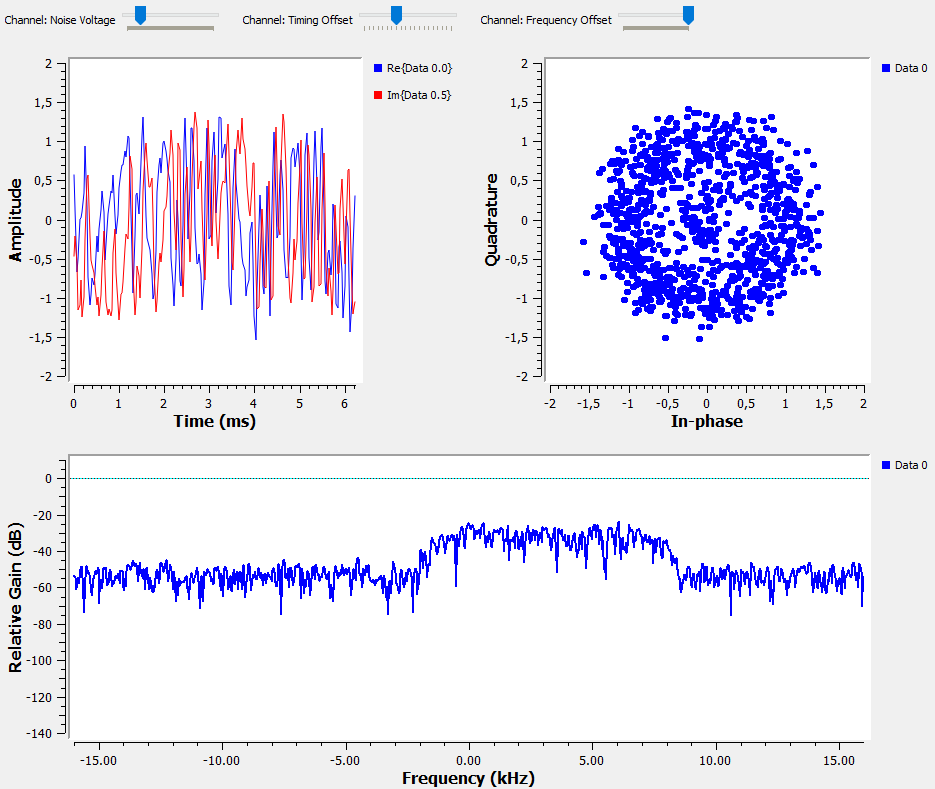
\includegraphics[width=0.8\linewidth]{resources/Images/task2_adding_channel_impairments}
        \caption{Добавление нарушений канала.}
        \label{fig:task2_mpsk_stage2}
    \end{figure}

    График созвездия показывает нам облако образцов, намного хуже того, с чего мы начали на последнем этапе.
    Теперь, исходя из полученного сигнала, мы должны отменить все эти эффекты.

    \newpage

    % --------------------------------------- Восстановление timing ----------------------------------------------
    \section{Восстановление timing}
    \label{sec:task3}

    Теперь изучим процесс восстановления.
    Существует множество алгоритмов восстановления, однако мы будем использовать алгоритм восстановления
    многофазных \texttt{clock}. 
    Попытаемся найти наилучшее время для дискретизации входящих сигналов, что позволит максимизировать отношение
    сигнал/шум (SNR) каждой выборки, а также уменьшить влияние межсимвольных помех (ISI).
    
    \subsection{Проблема ISI}
    \label{subsec:task3_isi}

    Для иллюстрации проблемы ISI изучим файл \texttt{symbol\_sampling.grc}.
    В нём создаётся четыре отдельных символа из единиц в строке, после чего они фильтруются.

    \begin{figure}[h]
        \centering
        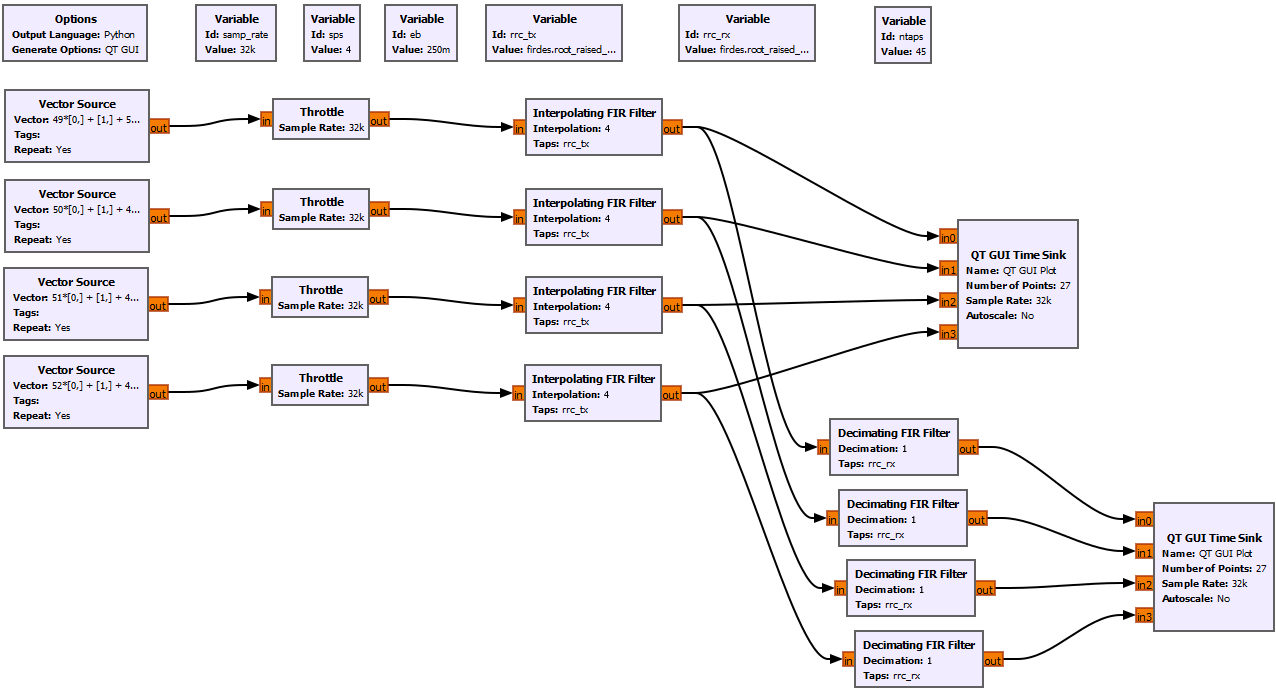
\includegraphics[width=0.9\linewidth]{resources/Images/task3_symbol_sampling}
        \caption{Flowgraph symbol\_sampling.grc}
        \label{fig:task3_symbol_sampling}
    \end{figure}

    \begin{figure}[h]
        \centering
        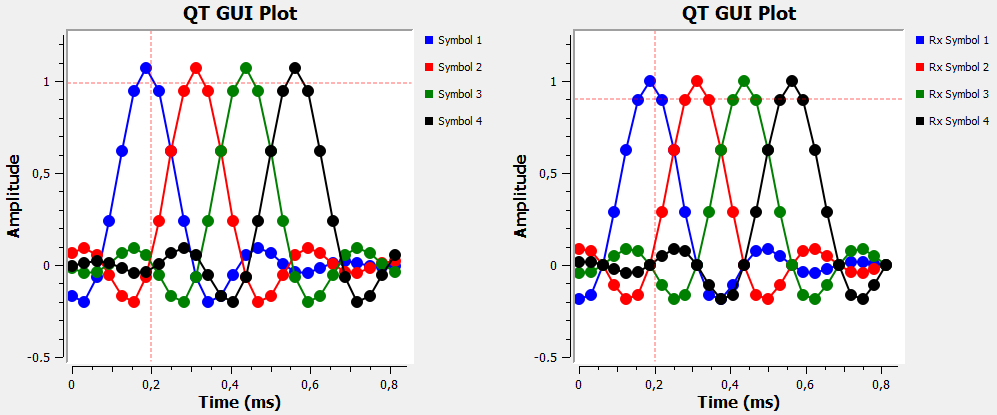
\includegraphics[width=0.8\linewidth]{resources/Images/task3_RRC_RC_filtered_symbols}
        \caption{Различия между символами, отфильтрованными RRC и RC.}
        \label{fig:task3_RRC_RC_filtered_symbols}
    \end{figure}

    На Рис.\ref{fig:task3_RRC_RC_filtered_symbols} можно увидеть различия между символами, отфильтрованными RRC и RC.
    Без фильтрации Найквиста в идеальной точке выборки каждого символа другие символы имеют некоторую энергию.
    Если мы сложим эти символы вместе, как в непрерывном потоке выборок, энергия этих других образцов складывается
    и искажает символ в этой точке.
    И наоборот, на выходе с RC-фильтром энергия от других отсчетов равна 0 в идеальной точке дискретизации
    для данного символа во времени.
    Это означает, что если мы делаем выборку в правильной точке выборки, мы получаем энергию только от
    текущего символа без помех от других символов в потоке.

    Это моделирование позволяет легко настраивать количество выборок на символ, избыточную полосу
    пропускания фильтров RRC и количество ответвлений.
    Мы можем поэкспериментировать с этими различными значениями, чтобы увидеть,
    как они влияют на поведение точки выборки.

    \newpage
    \subsection{Проблема разных clock}
    \label{subsec:task3_clock}

    Теперь рассмотрим влияние разных \texttt{clock} на точки выборки между передатчиком и приёмником.
    Для этого изучим файл \texttt{symbol\_sampling\_diff.grc}.

    Все \texttt{clock} несовершенны, поэтому начинаются в разный момент времени и дрейфуют относительно других \texttt{clock}.
    Смоделируем это, добавляя \texttt{resampler}, который немного регулирует время выборки символов между передаваемым
    сигналом и приёмником.

    \begin{figure}[h]
        \centering
        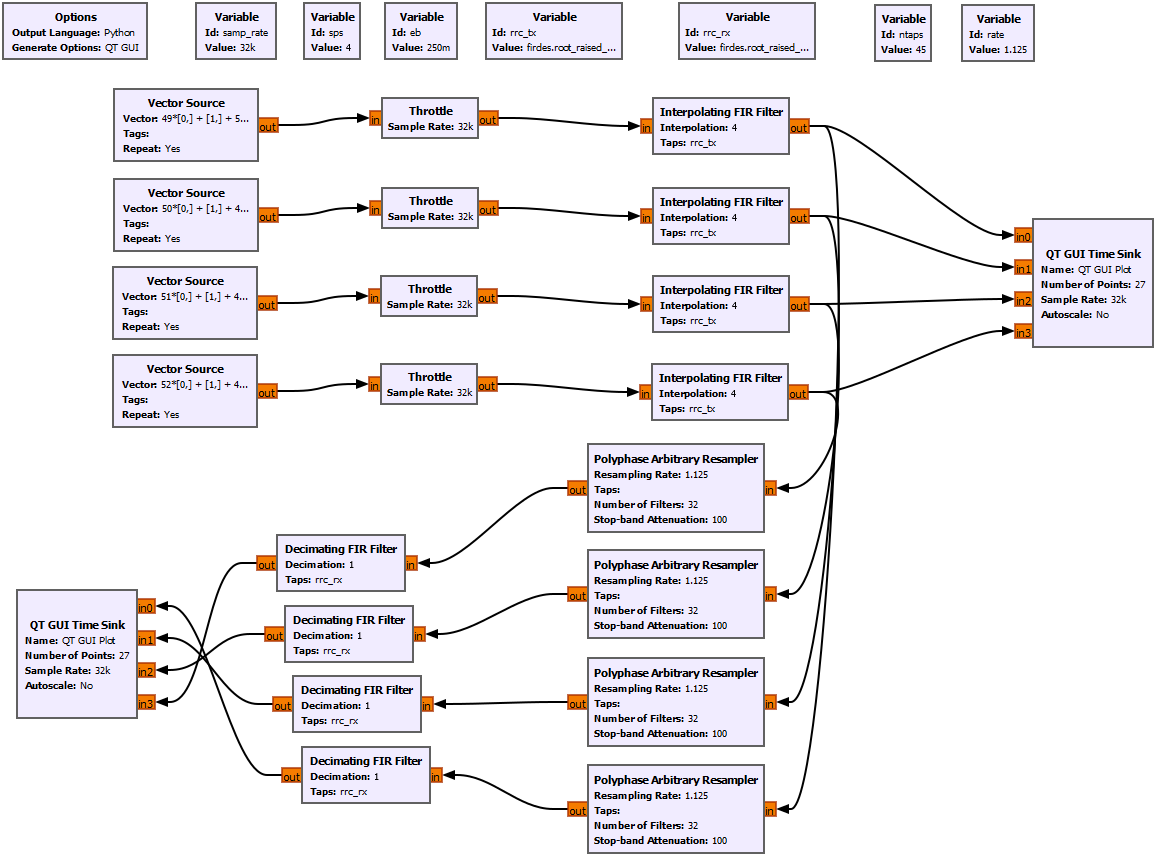
\includegraphics[width=0.8\linewidth]{resources/Images/task3_symbol_sampling_diff}
        \caption{Flowgraph symbol\_sampling\_diff.grc.}
        \label{fig:task3_symbol_sampling_diff}
    \end{figure}

    \begin{figure}[h]
        \centering
        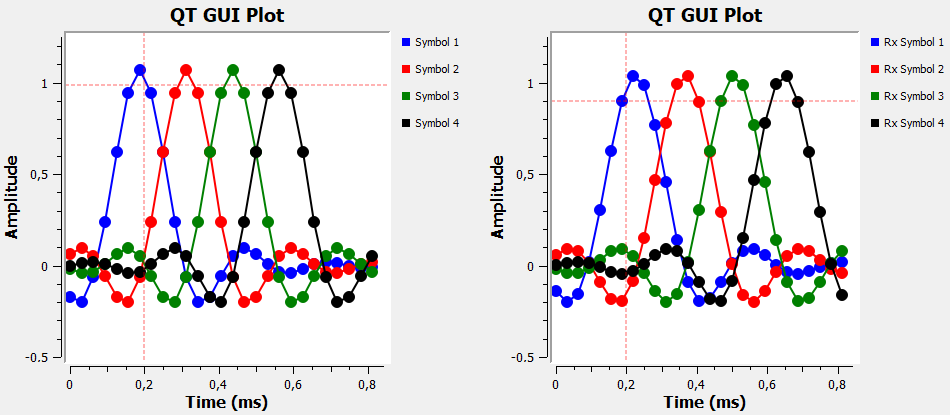
\includegraphics[width=0.8\linewidth]{resources/Images/task3_desynchronization}
        \caption{Передача четырёх символов с рассинхронизацией.}
        \label{fig:task3_desynchronization}
    \end{figure}

    Наша задача - синхронизировать \texttt{clock} передатчика и приёмника, используя только информацию в приёмнике из
    входящих выборок. Это задача восстановления \texttt{clock} или \texttt{timing}.

    \newpage
    \subsection{Блок синхронизации многофазных clock}
    \label{subsec:task3_clock_polyphase}

    Существуют различные алгоритмы для восстановления тактовой частоты на приёмнике.
    Мы будем использовать алгоритм восстановления \texttt{clock} многофазного блока фильтров.

    Этот блок делает 3 важные вещи:
    \begin{enumerate}
        \item Восстанавливает тактовую частоту.
        \item Согласует фильтр приёмника для устранения проблемы ISI.
        \item Выполняет понижающую дискретизацию сигнала и производит выборки со скоростью 1 sps.
    \end{enumerate}

    Итак, изучим файл \texttt{symbol\_differential\_filter.grc}.
    Нам нужен образец 0,22 мс.
    Фильтр разности ([-1, 0, 1]) генерирует дифференциал символа, и выходной сигнал этого фильтра в
    правильной точке выборки равен 0.
    Затем мы можем инвертировать этот оператор и вместо этого сказать, когда выход дифференциального
    фильтра равен 0, мы нашли оптимальную точку выборки.

    \begin{figure}[h]
        \centering
        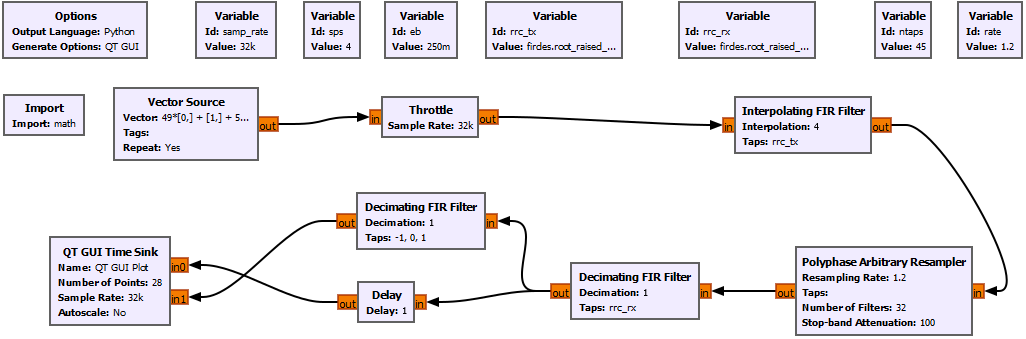
\includegraphics[width=0.9\linewidth]{resources/Images/task3_symbol_differential_filter}
        \caption{Flowgraph symbol\_differential\_filter.grc.}
        \label{fig:task3_symbol_differential_filter}
    \end{figure}

    Когда параметр скорости (\texttt{rate}) равен 1, смещения \texttt{clock} нет, а потому всё выглядит хорошо
    (Рис.\ref{fig:task3_without_clock_offset})

    \begin{figure}[H]
        \centering
        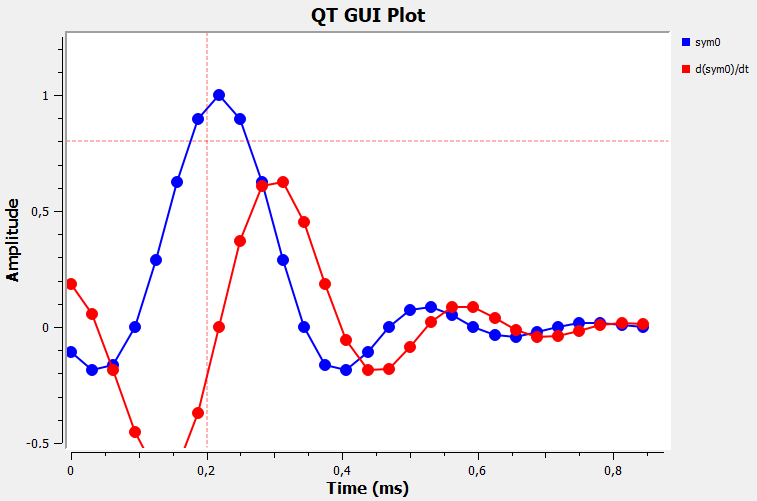
\includegraphics[width=0.8\linewidth]{resources/Images/task3_without_clock_offset}
        \caption{Без смещения clock (rate = 1).}
        \label{fig:task3_without_clock_offset}
    \end{figure}

    Теперь посмотрим, что происходит при смещении \texttt{timing}. Установим \texttt{rate = 1,2}.
    Результат можно увидеть на Рис.\ref{fig:task3_with_clock_offset}.

    \begin{figure}[H]
        \centering
        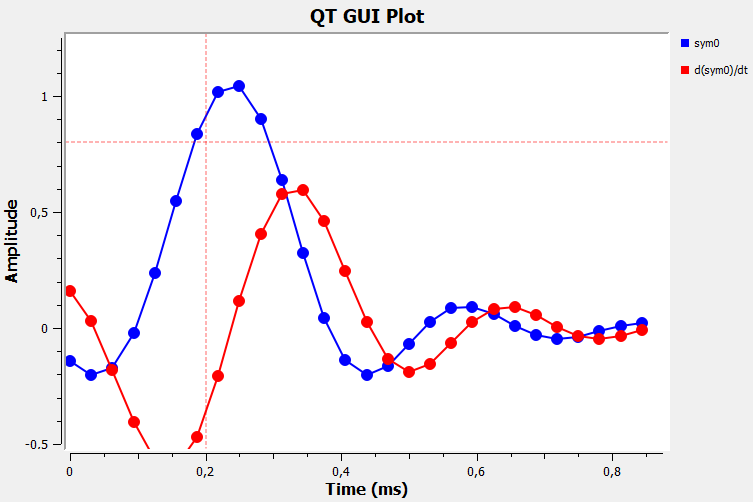
\includegraphics[width=0.8\linewidth]{resources/Images/task3_with_clock_offset}
        \caption{Со смещением clock (rate = 1,2).}
        \label{fig:task3_with_clock_offset}
    \end{figure}

    Можно заметить, что смещение \texttt{timing} происходит тогда, когда пик символа выключен,
    а производный фильтр не показывает нулевую точку.


    Вместо использования одного фильтра можно создать серию фильтров, каждый с разной фазой.
    При достаточном количестве фильтров на разных фазах, один из них имеет правильную фазу фильтра,
    которая даст нам желаемое значение синхронизации.

    Изучим файл \texttt{symbol\_differential\_filter\_phases.grc}.
    У нас есть 5 фильтров, что означает 5 различных фаз.

    \begin{figure}[h]
        \centering
        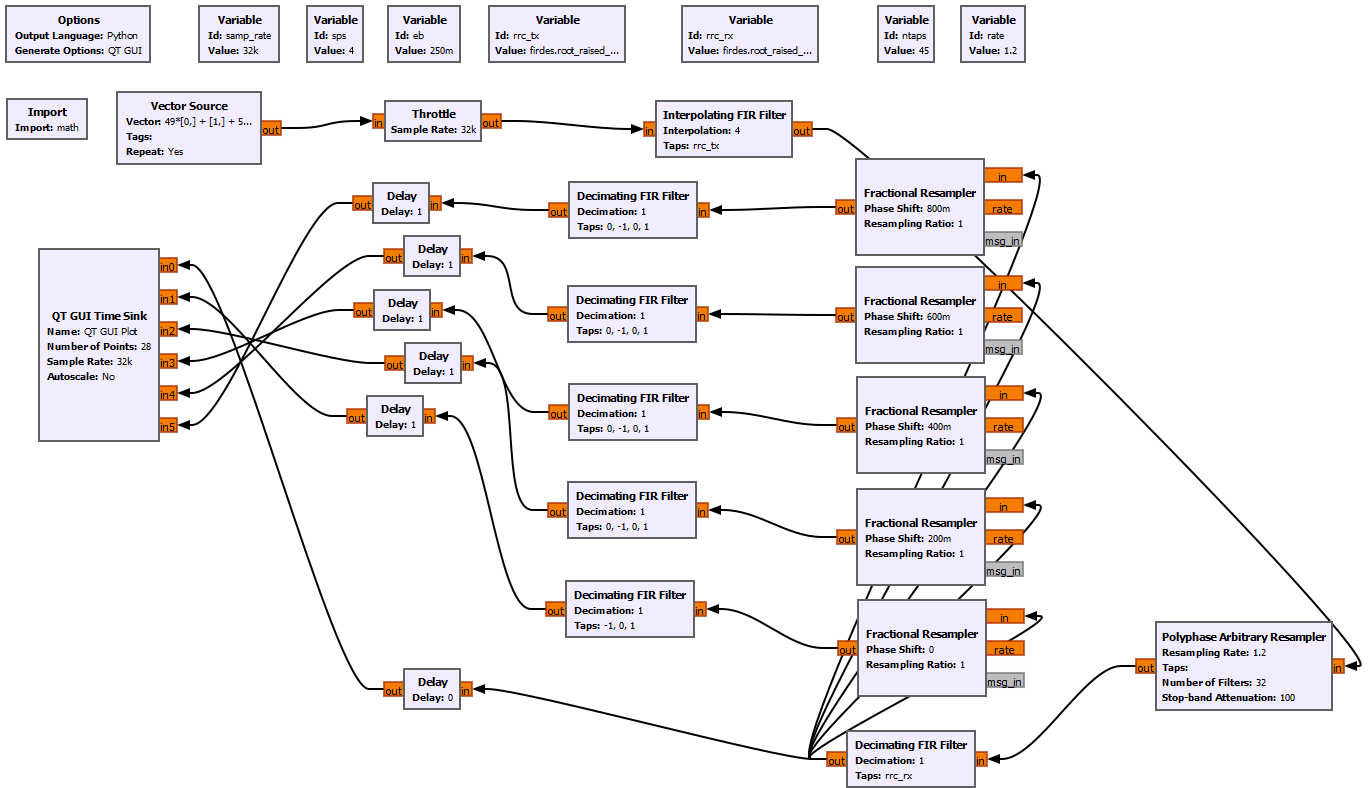
\includegraphics[width=0.8\linewidth]{resources/Images/task3_symbol_differential_filter_phases}
        \caption{Flowgraph symbol\_differential\_filter\_phases.grc.}
        \label{fig:task3_symbol_differential_filter_phases}
    \end{figure}

    \begin{figure}[h]
        \centering
        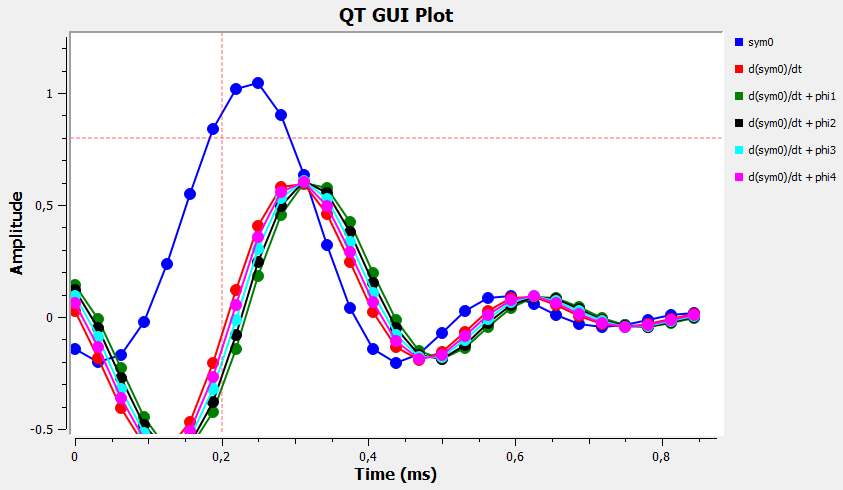
\includegraphics[width=0.8\linewidth]{resources/Images/task3_phases}
        \caption{Несколько фаз}
        \label{fig:task3_phases}
    \end{figure}

    На Рис.\ref{fig:task3_phases} видно, что сигнал \texttt{d(sym0)/dt + phi3} имеет точку отсчета в 0.
    Это говорит о том, что наша идеальная точка дискретизации находится при этом фазовом сдвиге.
    Следовательно, если мы возьмем RRC-фильтр нашего приемника и настроим его фазу на phi3
    (который составляет $3 * 2pi / 5$), то мы сможем исправить рассогласование по времени и выбрать
    идеальную точку дискретизации в это время дискретизации.

    Итак, мы использовали один из пяти фильтров в качестве идеальной точки дискретизации.
    Однако 5 фильтров недостаточно.
    Любое смещение выборки между этими фазами по-прежнему приведет к несвоевременной выборке с добавленным ISI.

    Давайте используем более 5 фильтров в нашем алгоритме восстановления тактовой частоты.
    Будем использовать 32 фильтра, чтобы получить максимальный коэффициент шума ISI,
    который меньше шума квантования 16-битного значения.

    \newpage
    \subsection{Использование блока многофазной синхронизации}
    \label{subsec:task3_using_clock_polyphase}

    Теперь используем блок многофазной синхронизации.
    Теперь давайте изучим файл \texttt{mpsk\_stage3.grc}.
    \texttt{Flowgraph} принимает выходные данные модели канала и передает их через наш блок Polyphase Clock Sync.
    Этот блок настроен с 32 фильтрами и полосой пропускания петли $2pi / 100$.

    \begin{figure}[h]
        \centering
        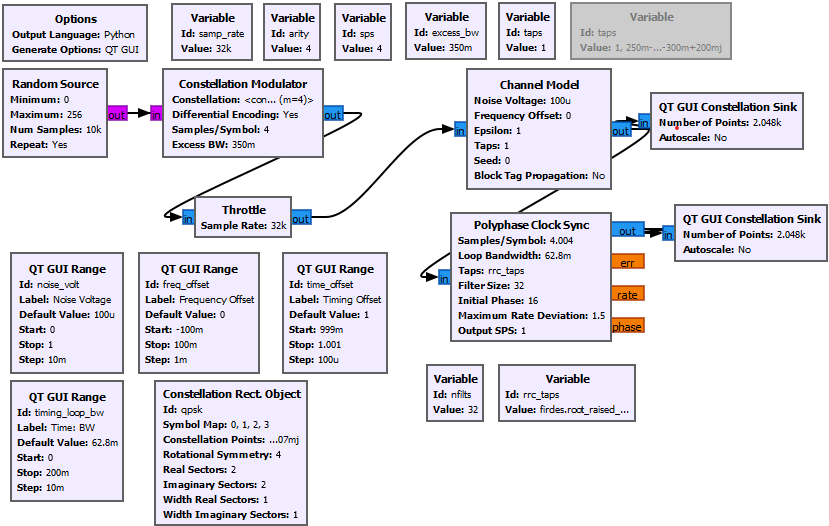
\includegraphics[width=0.8\linewidth]{resources/Images/task3_mpsk_stage3}
        \caption{Flowgraph mpsk\_stage3.grc.}
        \label{fig:task3_mpsk_stage3}
    \end{figure}

    \begin{figure}[h]
        \centering
        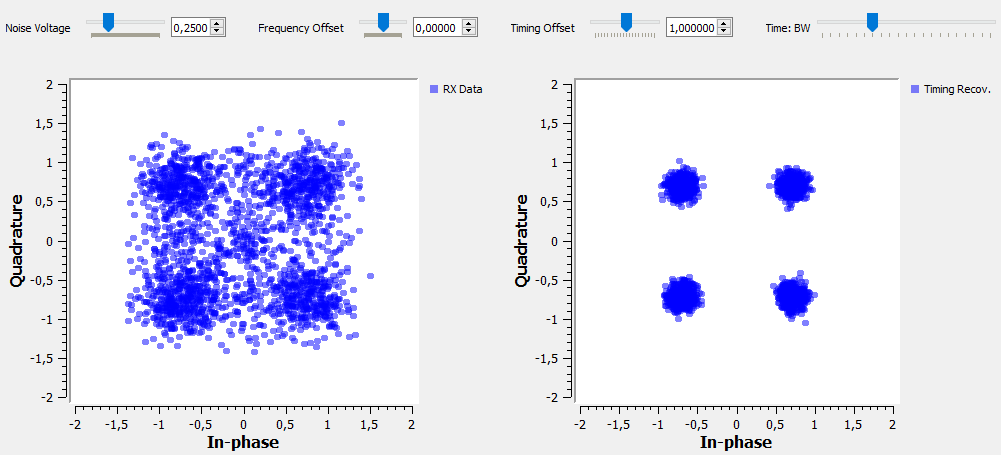
\includegraphics[width=0.8\linewidth]{resources/Images/task3_using_polyphase_clock_sync}
        \caption{Использование блока многофазной синхронизации.}
        \label{fig:task3_using_polyphase_clock_sync}
    \end{figure}

    На Рис.\ref{fig:task3_using_polyphase_clock_sync} мы видим дав созвездия: слева - полученный сигнал до
    восстановления синхронизации; справа - после восстановления синхронизации.
    Это все еще немного шумно из-за ISI.

    Мы также можем поэкспериментировать с изменением временного и частотного смещения.

    \newpage

    % --------------------------------------- Многолучевость ----------------------------------------------
    \section{Многолучевость}
    \label{sec:task4}

    Многолучевость - следствие того, что в большинстве коммуникационных сред у нас нет единственного
    пути для прохождения сигнала от передатчика к приемнику.
    Каждый раз, когда встречается объект, отражающий сигнал, между двумя узлами может быть установлен новый путь.
    Каждый из этих отражающих путей будет отображаться на приемнике в разное время в зависимости от длины
    пути. Суммирование их вместе в приемнике вызывает искажения, как конструктивные, так и деструктивные.

    Воздействие комбинации этих сигналов на приемник - искажение сигнала.
    Если разница во времени между отражениями мала по сравнению с шириной символа, искажение может быть
    внутри символа - внутрисимвольная интерференция.
    Если время отражения превышает время символа, отражение от одного символа будет влиять на следующие
    сигналы - еще одна причина межсимвольной интерференции.

    Изучим файл \texttt{multipath\_sim.grc}.

    \begin{figure}[h]
        \centering
        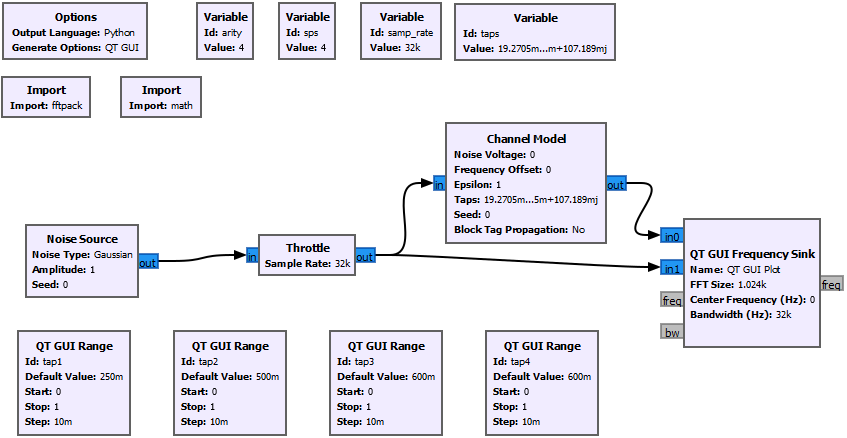
\includegraphics[width=0.9\linewidth]{resources/Images/task4_multipath_sim}
        \caption{Flowgraph multipath\_sim.grc.}
        \label{fig:task4_multipath_sim}
    \end{figure}

    В этом \texttt{flowgraph} происходит настройка модели канала таким образом, чтобы предоставить каналу
    пять элементов управления эквалайзером, четыре из которых мы можем изменить.
    Эти элементы управления настроены одинаково по частоте, и мы можем настроить их от 0 до 1.
    При значении 1 элемент управления позволит этим частотам проходить без помех.
    При значении 0 они создадут глубокий ноль в спектре, который повлияет на все частоты вокруг него.

    \begin{figure}[H]
        \centering
        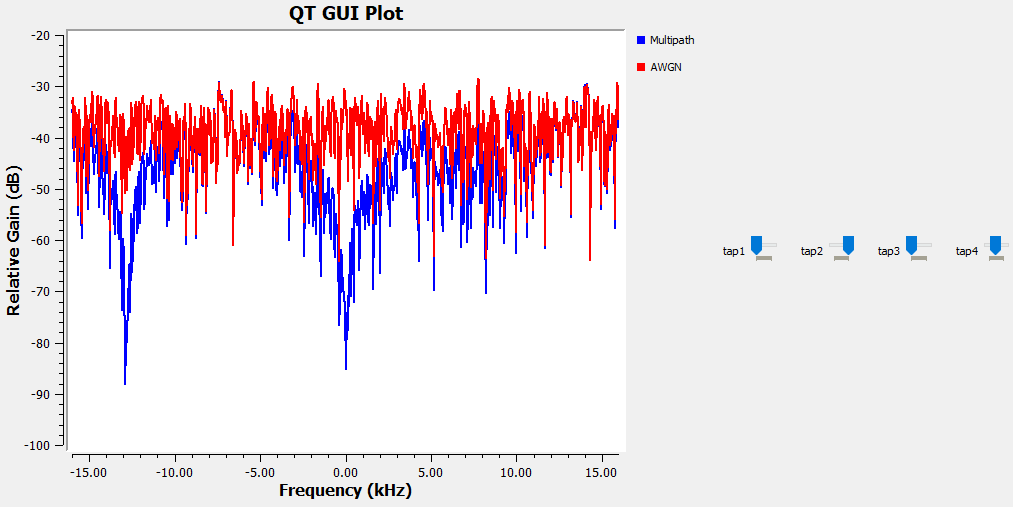
\includegraphics[width=0.9\linewidth]{resources/Images/task4_multipath_channel}
        \caption{Многолучевой канал.}
        \label{fig:task4_multipath_channel}
    \end{figure}

    Как видно на Рис.\ref{fig:task4_multipath_channel} многолучевой канал создает некоторые искажения в сигнале.
    Задача эквалайзера - инвертировать этот канал.
    По сути, мы хотим отменить искажение, вызванное каналом, чтобы выходной сигнал эквалайзера был ровным.
    Но вместо того, чтобы настраивать каждый tap вручную, можно использовать алгоритмы,
    которые обновляют эти tap за нас.
    Наша задача - использовать правильный алгоритм эквалайзера и настроить параметры.

    Одним из важных параметров здесь является количество tap в эквалайзере.
    Как мы видим в нашем моделировании, пять tap дают довольно грубый контроль над частотной характеристикой.
    Чем больше tap, тем больше времени требуется как на вычисление ответвлений,
    так и на запуск эквалайзера.

    \newpage

    % --------------------------------------- Эквалайзеры ----------------------------------------------
    \section{Эквалайзеры}
    \label{sec:task5}

    GNU Radio имеет два легко используемых эквалайзера: эквалайзер CMA и эквалайзер LMS-DD.

    \subsection{Эквалайзер CMA}
    \label{subsec:task5_cma}

     CMA или алгоритм постоянного модуля - это слепой эквалайзер , но он работает только с сигналами с
     постоянной амплитудой или модулем.
     Это означает, что цифровые сигналы, такие как MPSK, являются хорошими кандидатами,
     поскольку они имеют точки только на единичном круге.

     Изучим файл \texttt{mpsk\_stage4.grc}. В нём используется алгоритм CMA с 11 tap.

    \begin{figure}[h]
        \centering
        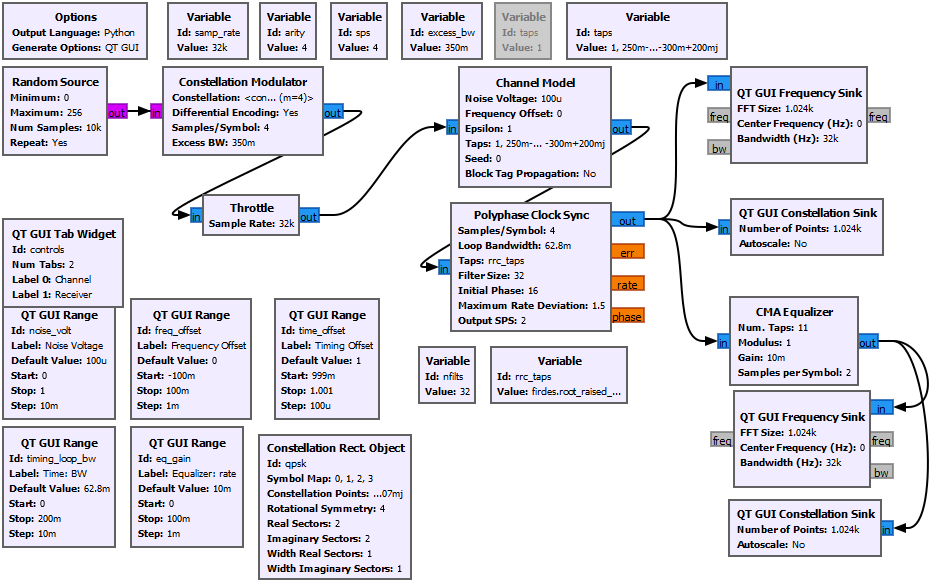
\includegraphics[width=0.9\linewidth]{resources/Images/task5_mpsk_stage4}
        \caption{Flowgraph mpsk\_stage4.grc.}
        \label{fig:task5_mpsk_stage4}
    \end{figure}

    На Рис.\ref{fig:task5_using_cma} можно видеть сходимость алгоритма CMA.
    Поскольку у нас есть и тактовая синхронизация, и блок эквалайзера, они сходятся независимо.
    В итоге мы можем увидеть эффект синхронизированного по времени многолучевого сигнала до и
    после эквалайзера.
    Перед эквалайзером у нас очень некрасивый сигнал даже без шумов.
    Эквалайзер прекрасно понимает, как инвертировать и сократить этот канал, чтобы у нас снова был хороший,
    чистый сигнал.

    \begin{figure}[H]
        \centering
        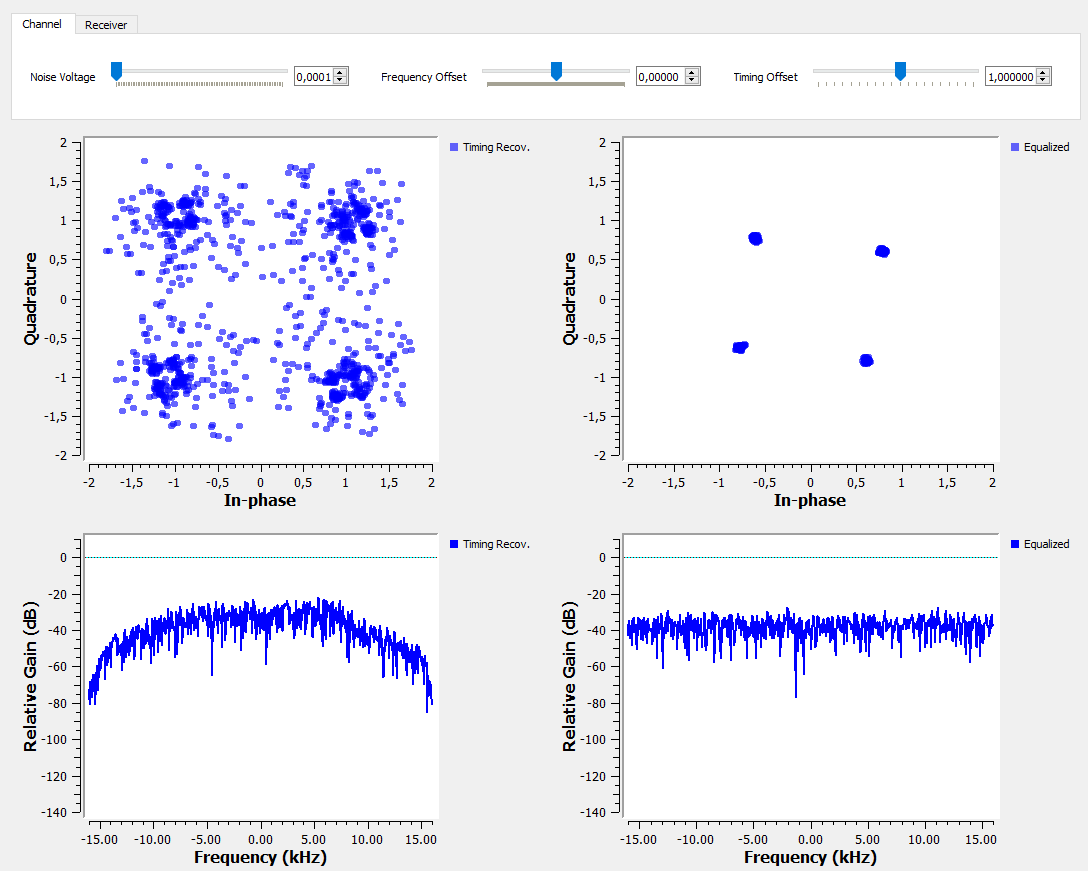
\includegraphics[width=0.9\linewidth]{resources/Images/task5_using_cma}
        \caption{Использование эквалайзера CMA.}
        \label{fig:task5_using_cma}
    \end{figure}

    \newpage
    \subsection{Эквалайзер LMS-DD}
    \label{subsec:task5_lms_dd}

    Эквалайзер LMS-DD - это эквалайзер, ориентированный на решение по алгоритму наименьшего среднего квадрата.
    В отличие от слепого эквалайзера (CMA), этот эквалайзер должен знать принимаемый сигнал.
    Эквалайзеру необходимо знать точки созвездия для корректировки, и он использует решения о выборках,
    чтобы сообщить, как обновлять ответвления для эквалайзера.

    Заменим эквалайзер CMA на эквалайзер LMS-DD в файле \texttt{mpsk\_stage4.grc}.

    \begin{figure}[H]
        \centering
        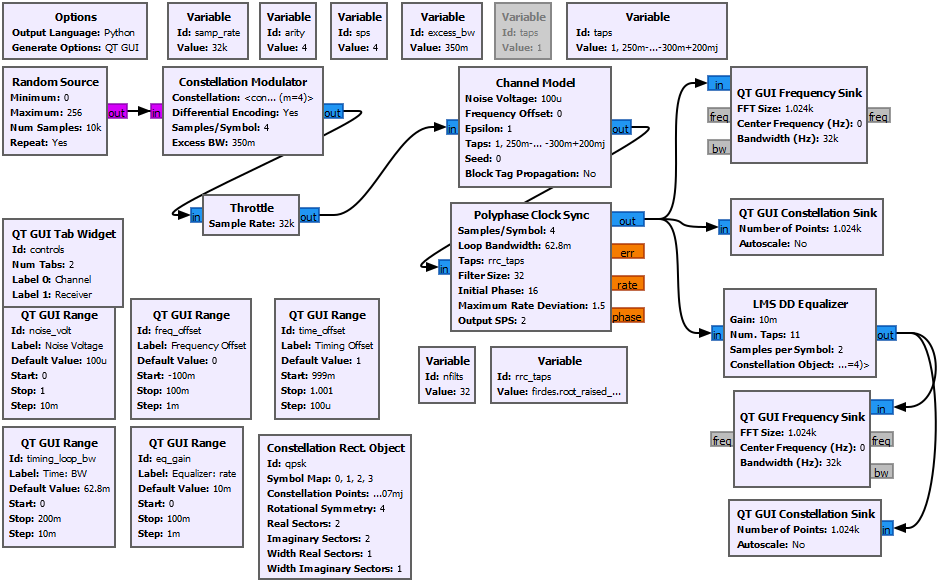
\includegraphics[width=0.7\linewidth]{resources/Images/task5_mpsk_stage4_lms_dd}
        \caption{Flowgraph mpsk\_stage4.grc с эквалайзером LMS-DD.}
        \label{fig:task5_mpsk_stage4_lms_dd}
    \end{figure}

    \begin{figure}[H]
        \centering
        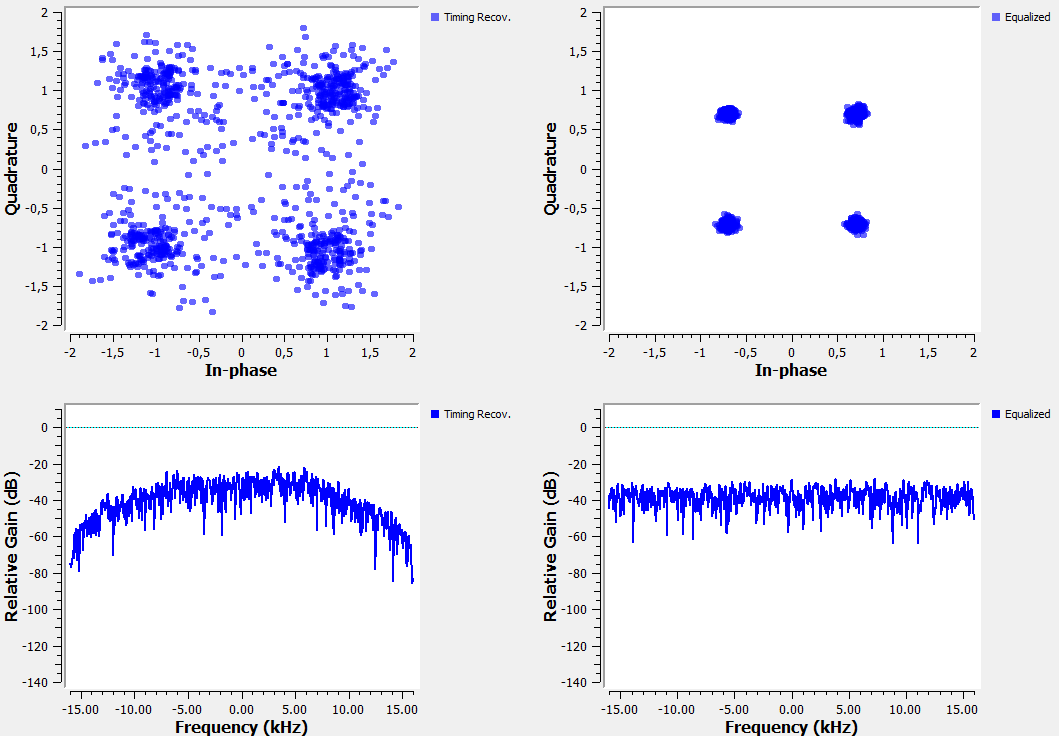
\includegraphics[width=0.7\linewidth]{resources/Images/task5_using_lms_dd}
        \caption{Использование эквалайзера LMS-DD.}
        \label{fig:task5_using_lms_dd}
    \end{figure}

    Этот эквалайзер отлично подходит для сигналов, которые не соответствуют требованиям постоянного модуля
    алгоритма CMA, поэтому он может работать с такими вещами, как модуляция типа QAM.
    Когда сигнал хорошего качества, этот эквалайзер может производить сигналы более высокого качества,
    потому что он напрямую знает сигнал.

    \newpage

    % --------------------------------------- Фазовая и точная частотная коррекция ----------------------------------------------
    \section{Фазовая и точная частотная коррекция}
    \label{sec:task6}

    Мы выровняли канал, однако у нас всё еще есть проблема смещения фазы и частоты.
    Эквалайзеры, как правило, адаптируются не быстро, поэтому смещение частоты может быть легко за
    пределами возможностей эквалайзера.
    Теперь нам нужно исправить любой сдвиг фазы, а также любой сдвиг частоты.

    Во-первых, мы будем использовать цикл второго порядка, чтобы мы могли отслеживать как фазу,
    так и частоту во времени.
    Во-вторых, тип восстановления, с которым мы будем иметь дело, предполагает, что мы выполняем точную
    коррекцию частоты.
    Поэтому мы должны находиться в приличном диапазоне идеальной частоты.

    Изучим файл \texttt{mpsk\_stage5.grc}. В нём используется цикл Костаса.

    \begin{figure}[h]
        \centering
        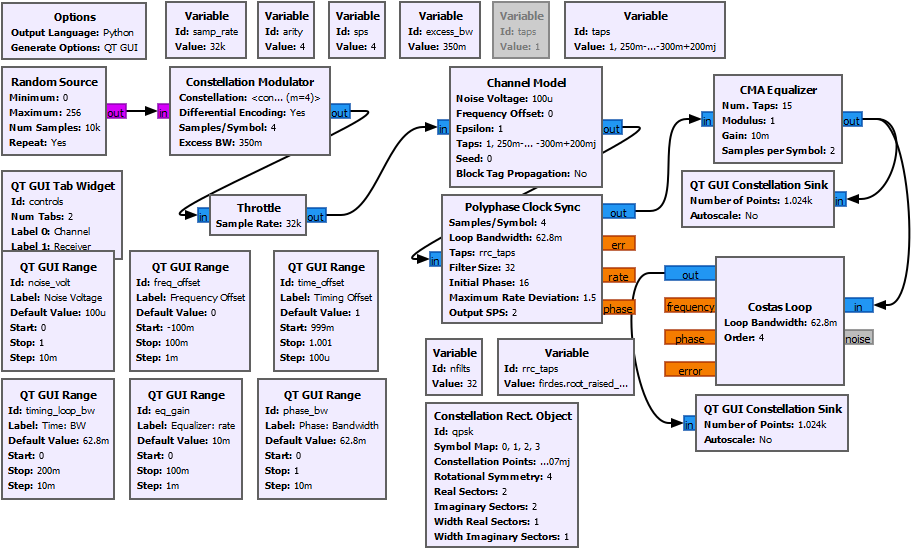
\includegraphics[width=0.9\linewidth]{resources/Images/task6_mpsk_stage5}
        \caption{Flowgraph mpsk\_stage5.grc.}
        \label{fig:task6_mpsk_stage5}
    \end{figure}

    Блок Costas Loop может синхронизировать BPSK, QPSK и 8PSK.
    Этот блок использует цикл второго порядка и поэтому определяется параметром полосы пропускания цикла.

    Мы установили шум, временной сдвиг, простой многолучевой канал и частотный сдвиг.
    После эквалайзера все символы находятся на единичном круге, но вращаются из-за смещения частоты,
    которое еще не исправлено.
    На выходе блока цикла Костаса можно увидеть заблокированное созвездие и дополнительный шум,
    с которым мы ничего не можем поделать.

    \begin{figure}[H]
        \centering
        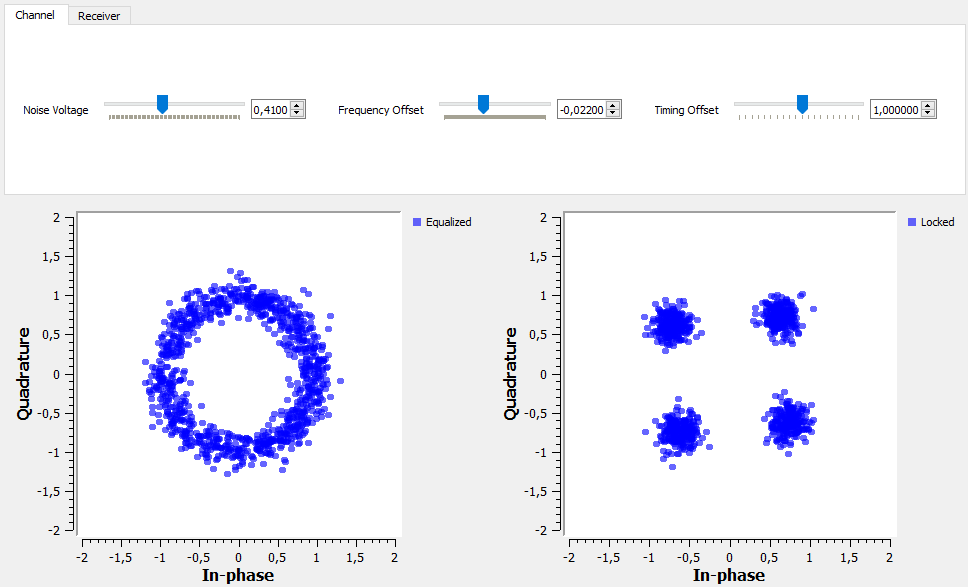
\includegraphics[width=0.9\linewidth]{resources/Images/task6_phase_freq_corr}
        \caption{Коррекция фазы и частоты.}
        \label{fig:task6_phase_freq_corr}
    \end{figure}

    \newpage

    % --------------------------------------- Расшифровка ----------------------------------------------
    \section{Расшифровка}
    \label{sec:task7}

    Теперь мы можем перейти к декодированию сигнала.
    Теперь давайте изучим файл \texttt{mpsk\_stage6.grc}.
    В этом \texttt{flowgraph} добавлен Constellation Decoder после цикла Костаса.
    Мы передавали дифференциальные символы, установив для параметра Differential в блоке
    Constellation Modulator значение True. Т.е., на самом деле мы передавали не само созвездие, а разницу
    между символами созвездия.

    \begin{figure}[h]
        \centering
        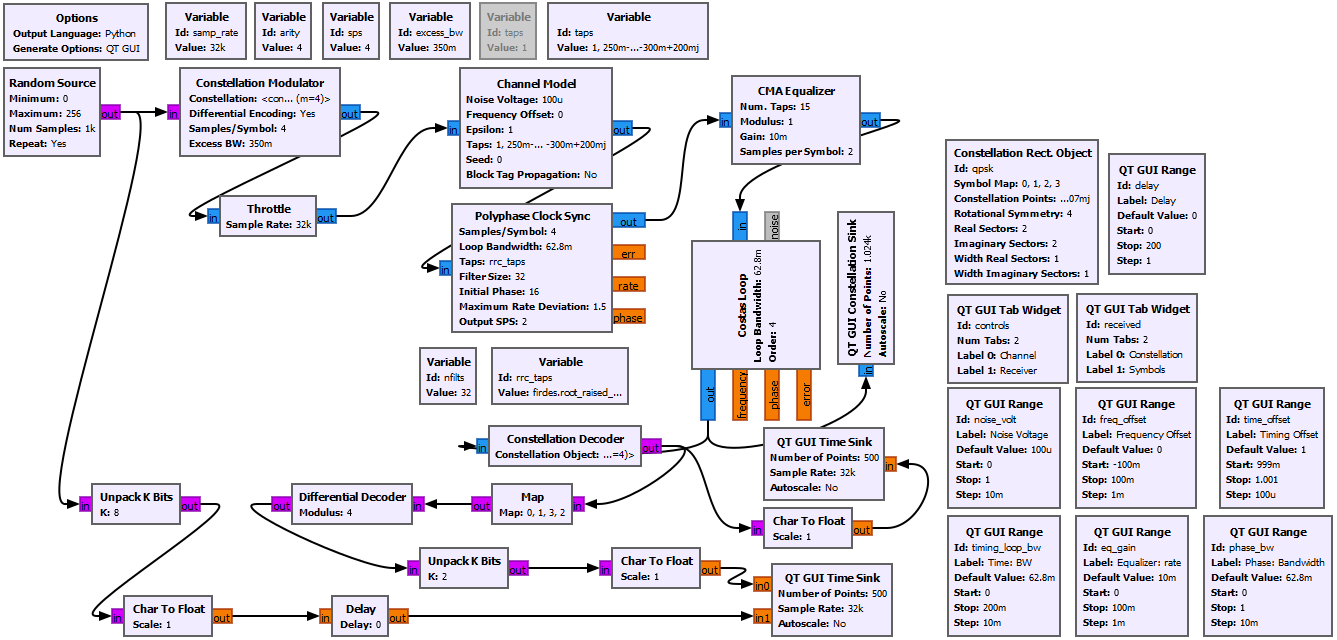
\includegraphics[width=0.9\linewidth]{resources/Images/task7_mpsk_stage6}
        \caption{Flowgraph mpsk\_stage6.grc.}
        \label{fig:task7_mpsk_stage6}
    \end{figure}

    В этом \texttt{flowgraph} используется блок Differential Decoder для преобразования кодированных
    дифференциальным кодом символов обратно в их исходные символы.
    Блок Map используется для преобразования символов из дифференциального декодера в исходные символы.
    Блок Unpack bits используется для распаковки исходных символов от 0 до 3 (2 бита на символ) в биты.
    Теперь у нас есть исходный битовый поток данных.

    Как мы узнаем, что это исходный битовый поток?
    Для этого сравним его с входным битовым потоком, но не напрямую.
    Необходимо установить задержку на переданные биты, используя Delay.
    Это связано с тем, что в цепочке приёмника есть множество блоков и фильтров, которые задерживают сигнал,
    а потому принятый сигнал отстаёт на некоторое количество бит.

    \begin{figure}[H]
        \centering
        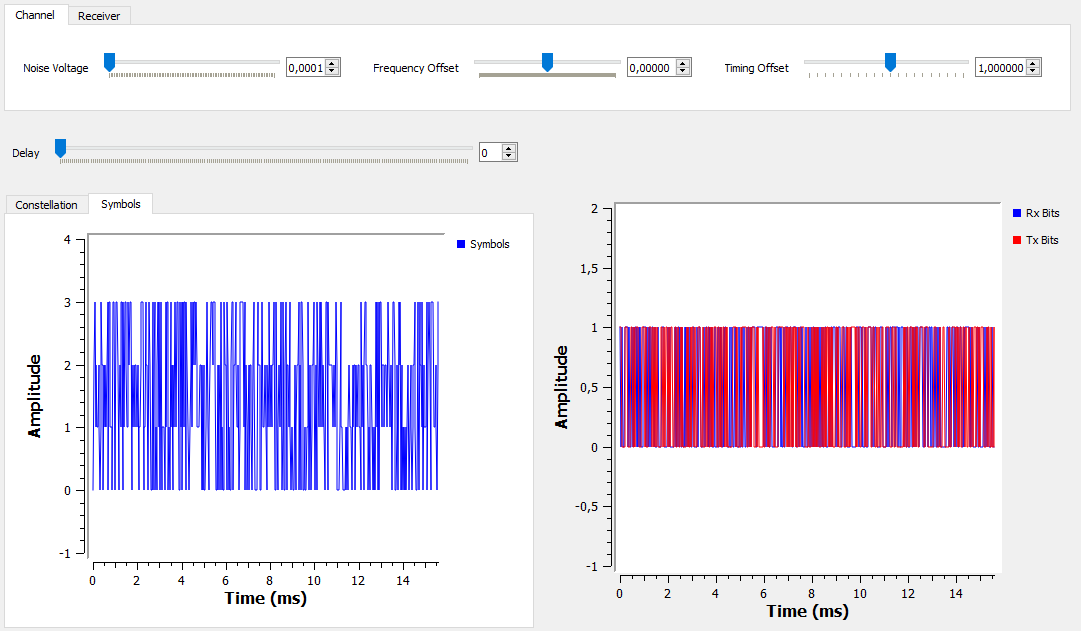
\includegraphics[width=0.9\linewidth]{resources/Images/task7_compare}
        \caption{Сравнение данных.}
        \label{fig:task7_compare}
    \end{figure}

 \newpage

% ---------------------------------------------- Выводы ----------------------------------------------
    \section{Выводы}
    \label{sec:conclusions}

    В ходе выполнения данной лабораторной работы была изучена демодуляция PSK.
    Были изучены проблемы искажения сигнала и эффектов канала.
    Также были изучены основные моменты, необходимые для восстановления сигнала:
    сроки восстановления, многолучевые каналы, фазовая и частотная коррекции, декодирование символов и
    порядок битов.

\end{document}